\chapter[Estado do arte]{Estado do Arte\label{estado_do_arte}}

Neste capítulo explicarase como funciona a internacionalización e localizacion con GNU Gettext. Ademais analizaremos as diferentes alternativas que existen no mercado como ferramentas de asistencia a tradución e as caracteristicas que cada unha incorpora. O final faremos un resumo das características que empregan os programas CAT\footnote{Computer Assisted Translation}.

\section{Internacionalización e localización con GNU Gettext}
Gettext é un sistema para a internacionalización e localización amplamente usado en entornos UNIX. Conta con varías implementacións, sendo a primira de Sun Microsystems no ano 1990. A implementación máis usada é a que GNU liberou no ano 1995. Pese ser unha solución antiga, é a día de hoxe a mellor que se pode atopar no mercado.

Para internacionalizar un programa con GNU Gettext non empregaremos as cadeas de texto directamente como podería ser no seguinte program de exemplo:

\begin{lstlisting}[language=C,label=some-code,caption=helloworld.c (Sen Internacionalizar)]
#include <stdio.h>

int
main ()
{
    printf ("Hello World!");
}
\end{lstlisting}

En lugar diso chamaremos a unha función especial que proporciona Gettext de nome \lstinline{gettext()} pero que é máis empregada a través do seu alias \lstinline{_()}. Ademais configuraremos o programa para que colla a tradución do idioma que queiramos. Desta forma o programa anterior quedaría:

\begin{lstlisting}[language=C,label=some-code,caption=helloworld.c]
#include <stdio.h>
#include <locale.h>
#include <libintl.h>

#define _(str) gettext(str)

#define

int
main ()
{
    setlocale (LC_ALL, "");
    bindtextdomain ("helloworld", "/usr/local/share/locale");
    textdomain ("helloworld");

    printf (_("Hello World!"));
}
\end{lstlisting}

A función \lstinline{gettext()} é a encargada de substituir a cadea orixinal pola tradución. Non obstante vemos que debemos configurar algunhas cousas antes de poder chamar á función.

En primeiro lugar debemos establecer a linguaxe que queremos empregar no programa. Para iso usamos a función \lstinline{setlocale()}. O primeiro argumento da función determina que parte do locale actual queremos modificar. Entre outras podemos atopar:

\begin{description}
    \item[LC\_ALL] Queremos cambiar todo.
    \item[LC\_ADDRESS] Queremos cambiar a forma de formatear os enderezos.
    \item[LC\_MESSAGES] Os mensaxes do programa.
    \item[LC\_NUMERIC] O formateado das cantidades non monetaias
    \item[LC\_TIME] O formateado de datas e horas.
\end{description}

Por ultimo especificamos o codigo de idioma ou no case de empregar a cadea baleira empregamos os valores das variables de entorno.

Os códigos de idioma empregan a normativa ISO 639 polo que son da forma $$language[\_territory][.codeset][@modifier]$$ Por exemplo o código do galego empregando codificación UTF8 é \lstinline{gl_ES.UTF-8}.

Ademais debemos indicarlle o programa onde ten que atopar as traducións. Para iso empregamos a función \lstinline{bindtextdomain()} que liga un nome de dominio a unha ruta dentro do sistema e a función \lstinline{textdomain()} que lle indica o programa cal é o nome de dominio que debe empregar. Un dominio é un conxunto de cadeas que se empregan nunha parte determinada dun programa. Cada dominio debe ter un nome de dominio unico para os dominios dentro dun programa.

Con estes parametros Gettext xa é capaz de atopar as traducións que no caso do programa anterior atoparíanse en \emph{/usr/local/share/locale/gl/LC\_MESSAGES/helloworld.mo}.

Unha vez que internacionalizamos o nosos programa debemos traducir as cadeas. Pero para traducir as cadeas debemos extraelas antes do código fonte. Para iso empregaremos a utilidade xgettext. Empregando as opcións adecuadas obtemos o seguinte ficheiro:

\begin{lstlisting}[label=some-code,caption=helloworld.pot]
# SOME DESCRIPTIVE TITLE.
# Copyright (C) YEAR THE PACKAGE'S COPYRIGHT HOLDER
# This file is distributed under the same license as the PACKAGE package.
# FIRST AUTHOR <EMAIL@ADDRESS>, YEAR.
#
#, fuzzy
msgid ""
msgstr ""
"Project-Id-Version: PACKAGE VERSION\n"
"Report-Msgid-Bugs-To: \n"
"POT-Creation-Date: 2014-11-12 19:24+0100\n"
"PO-Revision-Date: YEAR-MO-DA HO:MI+ZONE\n"
"Last-Translator: FULL NAME <EMAIL@ADDRESS>\n"
"Language-Team: LANGUAGE <LL@li.org>\n"
"Language: \n"
"MIME-Version: 1.0\n"
"Content-Type: text/plain; charset=CHARSET\n"
"Content-Transfer-Encoding: 8bit\n"

#: helloworld.c:14
#, c-format
msgid "Hello World!"
msgstr ""
\end{lstlisting}

Os ficheiros Gettext coa extensión \emph{pot} trátanse de plantillas xenéricas para todos os idiomas. Para obter o arquivo especifico para o noso idioma debemos empregar a ferramenta msginit con esta ferramenta obteremos un ficheiro similar a este:

\begin{lstlisting}[label=some-code,caption=helloworld.po (Sen Traducir)]
# Galician translations for HELLOWORLD package.
# Copyright (C) 2014 THE HELLOWORLD COPYRIGHT HOLDER
# This file is distributed under the same license as the ch package.
# Marcos Chavarría Teijeiro <chavarria1991@gmail.com>, 2014.
#
msgid ""
msgstr ""
"Project-Id-Version: ch 01\n"
"Report-Msgid-Bugs-To: \n"
"POT-Creation-Date: 2014-11-12 19:24+0100\n"
"PO-Revision-Date: 2014-11-12 19:54+0100\n"
"Last-Translator: Marcos Chavarría Teijeiro <chavarria1991@gmail.com>\n"
"Language-Team: Galician\n"
"Language: gl_ES\n"
"MIME-Version: 1.0\n"
"Content-Type: text/plain; charset=ISO-8859-1\n"
"Content-Transfer-Encoding: 8bit\n"

#: helloworld.c:14
#, c-format
msgid "Hello World!"
msgstr ""
\end{lstlisting}

Desta forma obtemos un ficheiro Gettext PO que é o archivo que temos que editar. Traducindo o arquivo obtemos algo como isto:

\begin{lstlisting}[label=lst:translated_example,caption=helloworld.po (Traducido)]
# Galician translations for HELLOWORLD package.
# Copyright (C) 2014 THE HELLOWORLD COPYRIGHT HOLDER
# This file is distributed under the same license as the HELLOWORLD package.
# Marcos Chavarría Teijeiro <chavarria1991@gmail.com>, 2014.
#
msgid ""
msgstr ""
"Project-Id-Version: HELLOWORLD 1.0\n"
"Report-Msgid-Bugs-To: \n"
"POT-Creation-Date: 2014-11-12 19:24+0100\n"
"PO-Revision-Date: 2014-11-12 19:54+0100\n"
"Last-Translator: Marcos Chavarría Teijeiro <chavarria1991@gmail.com>\n"
"Language-Team: Galician\n"
"Language: gl_ES\n"
"MIME-Version: 1.0\n"
"Content-Type: text/plain; charset=ISO-8859-1\n"
"Content-Transfer-Encoding: 8bit\n"

#: helloworld.c:14
#, c-format
msgid "Hello World!"
msgstr "Ola Mundo!"
\end{lstlisting}

Antes de poder empregar o ficheiro no noso programa temos que compilalo. Para iso empregamos a utilidade msgfmt ca que obtemos o ficheiro helloworld.mo. Se movemos o ficheiro o directorio adecuado (o que especificamos en \lstinline{textdomain()}) o noso programa xa estará localizado.

%http://www.gnu.org/software/libc/manual/html_node/Locating-gettext-catalog.html

\subsection{Ficheiros Gettext PO}
Como xa dixemos antes os ficheiros PO son os ficheiros que temos que editar para localizar o noso programa. Primeiro dicir que se trata ficheiros de texto plano e que polo tanto podemos editar con calquer editor de ficherios de texto plano.

As súas principais características son:

\paragraph{Soporte de plurales}
Algo que pode parecer trivial como o soporte de plurales deixa de selo cando consideramos que non todos as linguaxes do mundo empregan dous plurales. A lingua eslovaca, por exemplo, conta con tres formas de plural de forma que o plural faise diferente para 1, 3 e 5 elementos.

Gettext representa a forma de plural de cada linguaxe con unha cadea da seguinte forma: $$nplurals=n; plural=exp;$$ Onde $n$ representa o número de plurais da linguaxe e $exp$ a expresión para calcular cando debemos empregar cada forma.

\paragraph {Marcado de traducións difusas}
Permitese marcar certas traducións como difusas de forma que o traductor indica qu enon está seguro de que dita tradución sexa correcta.

\paragraph {Formato das traducións}
Os ficheiro po permite indicar se as cadeas a traducir teñen un formato determinado. Por exemplo a cadea do exemplo no Fragmento de Código \ref{lst:translated_example} podese ver que ten o flag \lstinline{c-format} debido a que é parte dunha sentencia printf e podería levar indicadores de formato da forma \lstinline{%s}.

\paragraph {Cabeceira con metadatos}
Exite unha cadea especial nos documentos Gettext PO. Trátase da cadea baleira que serve para almacenar metadatos do ficheiro. Almacenase o id do proxecto, o idioma do ficheiro, a data da última tradución e o nome e apelidos de quen a fixo entre outros moitos datos. No fragmento de código \ref{lst:translated_example} podemos ver estos campos.

\paragraph{Gardado dos orixes das cadeas}
Gettext almacena para cada cadea en que lugares do código aparece esta. O cal pode ser moi interesante para implentar a previsualización das traducións.

\paragraph{Comentarios dos programadores}
É unha función moi importante xa que en moitas ocasións nas linguaxes a mesma palabra empregase como verbo ou como nome polo que en ocasións é importante incorporar un contexto para esa tradución.

\paragraph{Comentarios dos traductores}
A biblioteca permite que os traductores comenten as cadeas.

\section{Ferramentas CAT do mercado}

Nesta sección repasaremos as alternativas existentes no mercado.

\subsection{GTranslator}
GTranslator é a aplicación oficial do proxecto GNOME para a asistencia a tradución. Este aplicativo so permite a tradución de arquivos GNU Gettext. As característica máis destacables deste programa son a posibilidade de abrir varios ficheiros en diferentes lapelas, soporte de memorias de tradución, perfiles para diferentes traductores, edición dos comentarios dos ficheiros .po e un sistema de plugins que permite extender a ferramenta.

\begin{figure}[h]
    \centering
    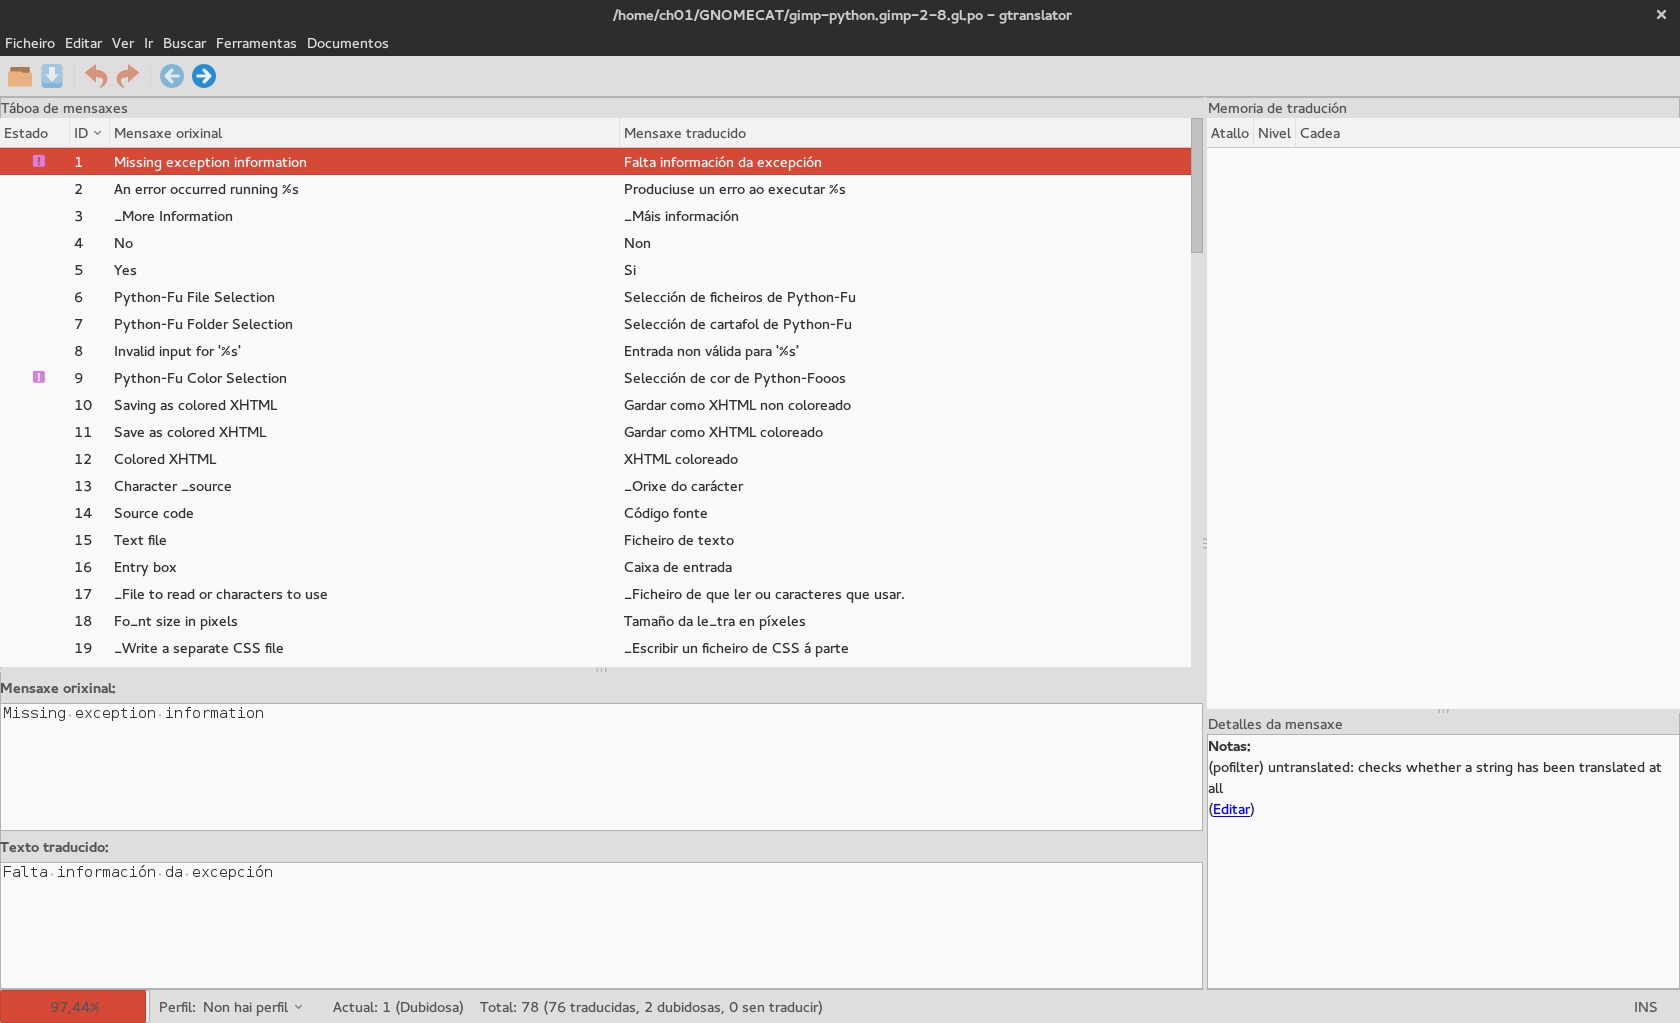
\includegraphics[width=\textwidth]{img/captura_gtranslator.png}
    \caption[Interface de GTranslator]{Interface de GTranslator}
    \label{fig:gtranslator}
\end{figure}

En canto a interface, como podemos ver na Figura~\ref{fig:granslator}, a parte máis importante do programa é a a lista de mensaxes. Abaixo temos un panel onde se pode editar cada mensaxe e a dereita a memoria de tradución. O programa tamén incorpora atallos de teclado que permiten moverse polo documento e selecionar cada elemento da memoria de tradución.

Este programa pese a ser o aplicativo oficial de GNOME é moi pouco usado. As razóns disto son a ausencia dunha característica chave que o diferencie doutras ferramentas do mercado, a presencia de fallas importantes que afectan a usabilidade e a ausencia dun mantenedor que resolva estos problemas.

\subsection{Lokalize}
Lokalize é o programa oficial para a tradución en KDE. Ten soporte para ficheiros GNU Gettext e para Qt ts (o formato propio de KDE) entre outros. Entre as caracteristicas a destacar é o soporte para proxectos de tradución cunha panel resumo de tod o contido de cada proxecto, ten glosario, memoria de tradución, posibilidade de ver os propios ficheiros fonte desde a interface a través de scripts feitos polo traductor, multiples perfiles, etc.

\begin{figure}[h]
    \centering
    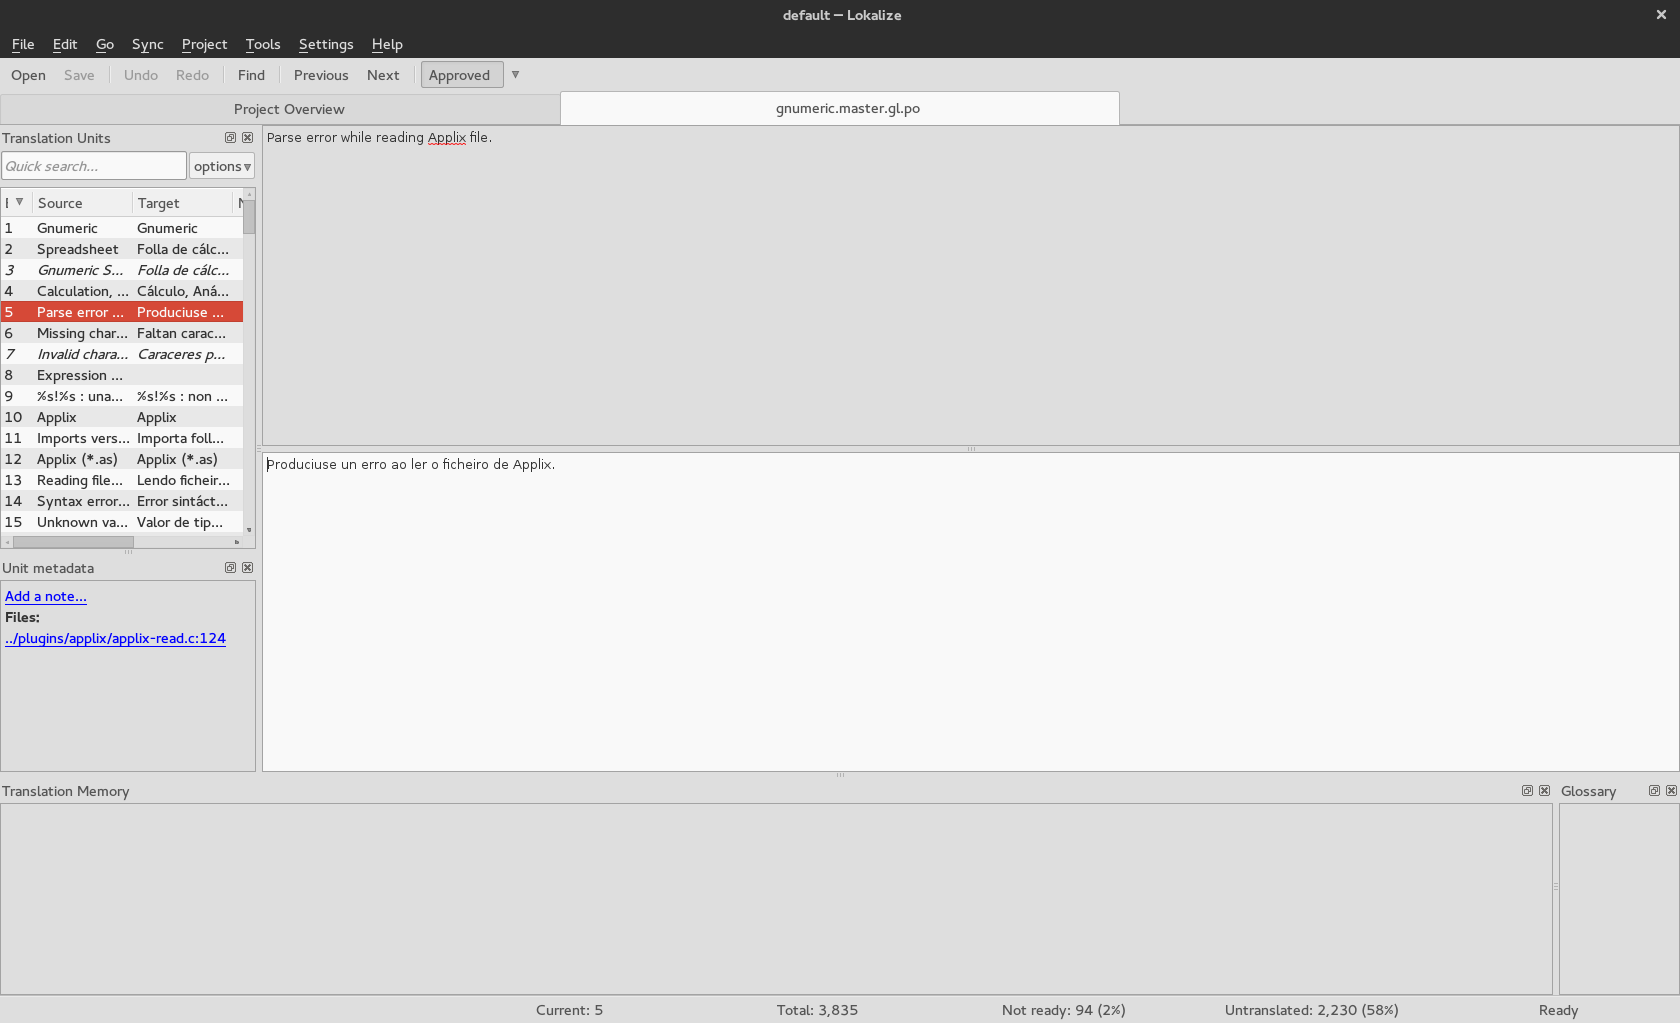
\includegraphics[width=\textwidth]{img/captura_lokalize.png}
    \caption{Interface de Lokalize}
    \label{fig:lokalize}
\end{figure}


\subsection{Virtaal}

Vitaal é unha ferramenta CAT creada por Translate House.

\begin{figure}[h]
    \centering
    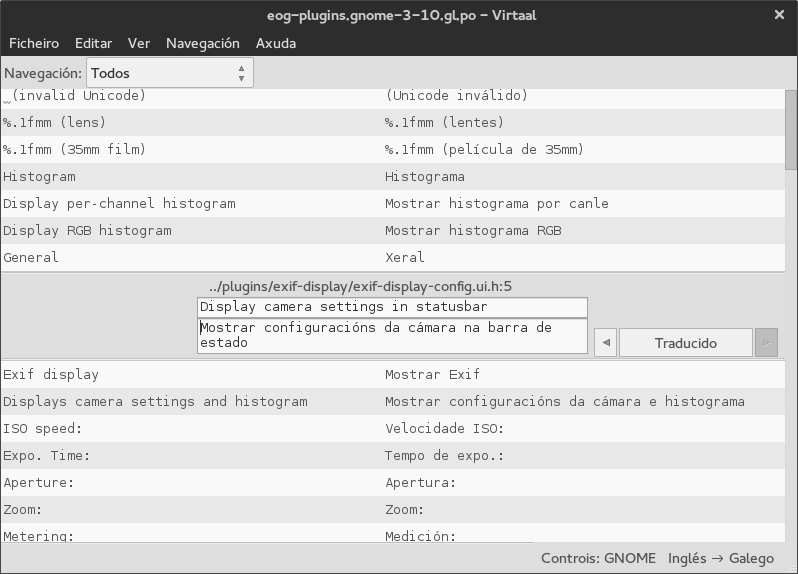
\includegraphics[width=\textwidth]{img/captura_virtaal.png}
    \caption{Interface de Virtaal}
    \label{fig:virtaal}
\end{figure}

\subsection{OmegaT}

\subsection{Google Translation Toolkit}
Metras que todas as solucións anteriores eran solucións de escritorio, Google Translation Toolkit é unha ferramenta web desenvolvida por Google.

\begin{figure}[h]
    \centering
    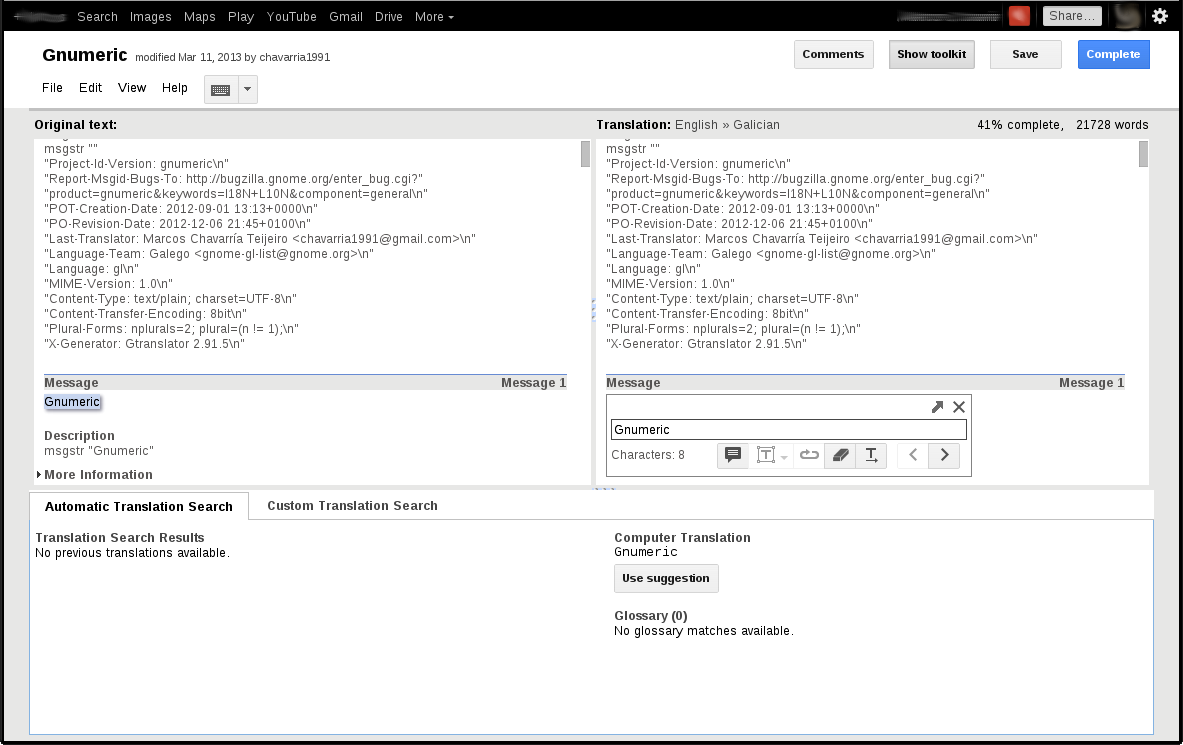
\includegraphics[width=\textwidth]{img/captura_googletranslationtoolkit.png}
    \caption{Interface de Google Translation Toolkit}
    \label{fig:translatetoolkit}
\end{figure}

\subsection{Transifex}
Tamén se trata dunha solución web. Neste caso de pago.

\begin{figure}[h]
    \centering
    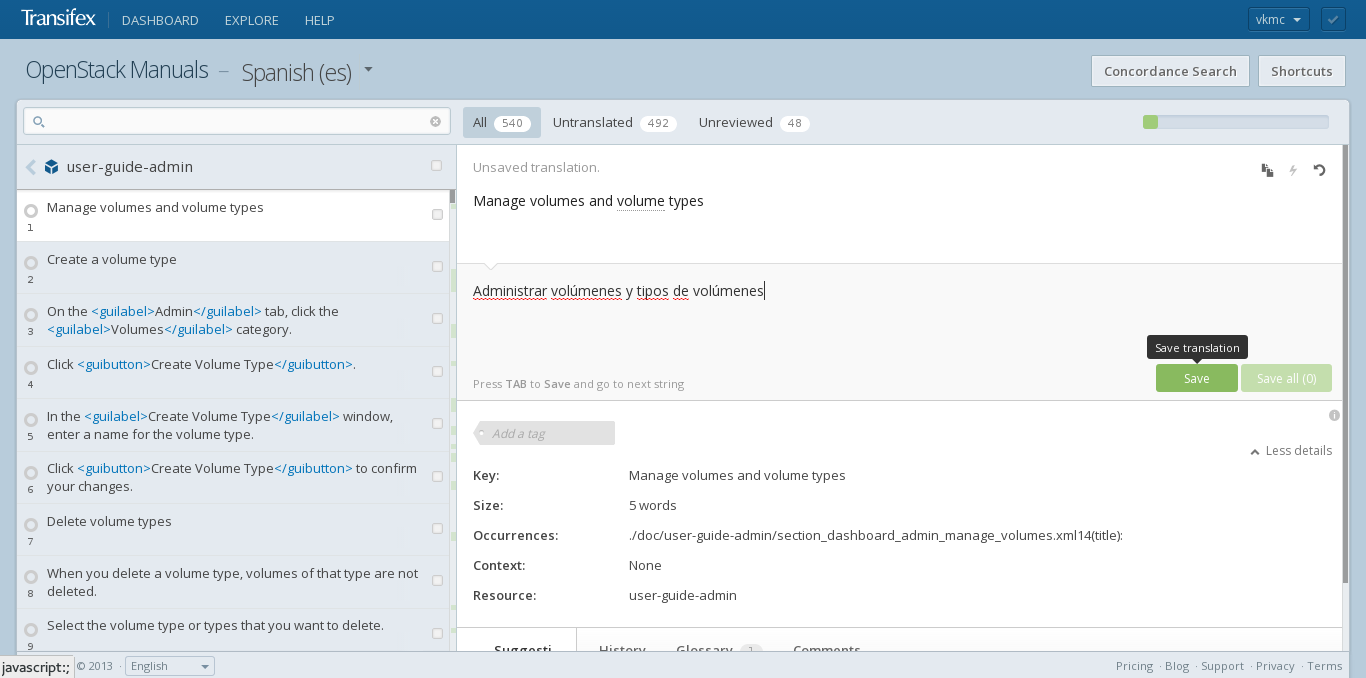
\includegraphics[width=\textwidth]{img/captura_transifex.png}
    \caption{Interface de Transifex}
    \label{fig:transifex}
\end{figure}


%
% FIN DEL CAPÍTULO
%